\documentclass[9pt,aspectratio=169]{beamer}


\usepackage{tabu, booktabs, multirow}
\usepackage{tabularx}
\usepackage{multicol}
\usepackage{setspace}
\usepackage[official]{eurosym}
\usepackage{graphicx}

\usepackage{hyperref}
\hypersetup{
    colorlinks=true,
    linkcolor=blue,
    filecolor=magenta,      
    urlcolor=cyan,
    pdftitle={EC3318/MN3101 Lecture 2},
    pdfpagemode=FullScreen,
    }

\urlstyle{same}

\graphicspath{ {./pix_l2/} }



\newcolumntype{Y}{>{\centering\arraybackslash}X}  % Centered version of X

\newcommand{\placeholderbox}[1]{%
  \begin{center}
    \fbox{\parbox[c][0.5\textheight][c]{0.9\linewidth}{\centering \textit{#1}}}
  \end{center}
}
% St Andrews Color Palette

% Blues
\definecolor{StAndrewsLightBlue}{RGB}{0,174,239}
\definecolor{StAndrewsMidBlue}{RGB}{0,125,197}
\definecolor{StAndrewsBlue}{RGB}{0,83,155}  % Previously defined

% Reds
\definecolor{StAndrewsBurgundy}{RGB}{198,12,70}
\definecolor{StAndrewsRed}{RGB}{238,49,42}  % Previously defined

% Purple
\definecolor{StAndrewsPurple}{RGB}{123,67,154}

% Orange
\definecolor{StAndrewsOrange}{RGB}{245,132,43}

% Greens
\definecolor{StAndrewsGreen}{RGB}{84,185,72}
\definecolor{StAndrewsMidGreen}{RGB}{0,133,63}
\definecolor{StAndrewsDarkGreen}{RGB}{0,89,83}

% Yellow
\definecolor{StAndrewsYellow}{RGB}{255,223,0}

% Black
\definecolor{StAndrewsBlack}{RGB}{35,31,32}

\setbeamercolor*{structure}{fg=StAndrewsBlack}
\setbeamercolor{title}{fg=StAndrewsBlack}
\setbeamercolor{title separator}{fg=StAndrewsBlue}
\setbeamercolor{frametitle}{bg=StAndrewsBlue, fg=white}

\usetheme{metropolis}
\usepackage{tikz}
\usetikzlibrary{calc}
\usetikzlibrary{arrows.meta, positioning, shapes.geometric, shadows}
\usepackage[export]{adjustbox}
\usepackage{hyperref}
\hypersetup{
  colorlinks=true,
  linkcolor=StAndrewsBlue,
  urlcolor=StAndrewsBlue,
  citecolor=StAndrewsBlue
}

% Show a full-width colored header with title + subtitle
\setbeamercolor{frametitle}{bg=StAndrewsBlue, fg=white}
\setbeamercolor{framesubtitle}{fg=white}
\setbeamerfont{frametitle}{size=\Large,series=\bfseries}
\setbeamerfont{framesubtitle}{size=\small}
\setbeamerfont{title}{series=\mdseries}

\makeatletter
\setbeamertemplate{frametitle}{
  \nointerlineskip
  \begin{beamercolorbox}[wd=\paperwidth,sep=0.8ex,leftskip=1.2em,rightskip=1.2em]{frametitle}
    \usebeamerfont{frametitle}\strut\insertframetitle\par
    \ifx\insertframesubtitle\@empty\else
      \vspace{0.25ex}
      {\usebeamerfont{framesubtitle}\usebeamercolor[fg]{framesubtitle}\insertframesubtitle\par}
    \fi
  \end{beamercolorbox}
}
\makeatother

\makeatletter
\setbeamertemplate{title page}{
  \begin{minipage}[c][\textheight][c]{\textwidth}
    \centering
    \ifx\inserttitle\@empty\else\usebeamertemplate*{title}\fi
    \ifx\insertsubtitle\@empty\else\usebeamertemplate*{subtitle}\fi
    \vspace{8pt}
    {\usebeamercolor[fg]{title separator}\rule{0.72\textwidth}{0.4pt}\par}
    \vspace{10pt}
    \ifx\beamer@shortauthor\@empty\else\usebeamertemplate*{author}\fi
    \vspace{12pt}
    \ifx\insertinstitute\@empty\else\usebeamertemplate*{institute}\fi
    \vspace{6pt}
    \ifx\insertdate\@empty\else\usebeamertemplate*{date}\fi
    \vspace{9pt}
    \ifx\inserttitlegraphic\@empty\else\usebeamertemplate*{title graphic}\fi
  \end{minipage}
}

\setbeamertemplate{title}{
%  \raggedright%  % <-- Comment here
  \linespread{1.0}%
  \inserttitle%
  \par%
}
\setbeamertemplate{subtitle}{
%  \raggedright%  % <-- Comment here
  \insertsubtitle%
  \par%
  \vspace*{0.5em}
}
\setbeamertemplate{author}{
%  \raggedright%  % <-- Comment here
  \insertauthor%
  \par%
}
\setbeamertemplate{institute}{\insertinstitute\par}
\makeatother

\title{\LARGE Lecture 2: \\
Discount factors and cost of capital}
\author[Dr Christian Engels]{Dr Christian Engels}
\institute{\small{EC3318 Financial Economics: Corporate Finance \\ MN3101 Corporate Finance and Control \\[2mm] University of St Andrews Business School}}
\date{22 September 2026}


\newenvironment{wideitemize}{\itemize\addtolength{\itemsep}{10pt}}{\enditemize}
\setbeamertemplate{items}[circle]

\setbeamertemplate{title graphic}{\inserttitlegraphic\par}
\titlegraphic{
\includegraphics[scale=0.08]{logos/01-standard-black-text.png}}

% Add the logo to the bottom left
\addtobeamertemplate{footline}{%
  \begin{tikzpicture}[remember picture,overlay]
    \node[anchor=south west, inner sep=0pt] at ([xshift=0.5cm, yshift=0.25cm]current page.south west) {
      
\includegraphics[height=0.5cm]{logos/st-andrews-icon.png}
    };
  \end{tikzpicture}%
}{}

\usepackage{pgfplots}
\pgfplotsset{compat=1.18}
\usepgfplotslibrary{fillbetween}
\newcommand{\LBarrickMean}{3.1}
\newcommand{\LBarrickVar}{0.02473}
\newcommand{\LBarrickSD}{15.7}
\newcommand{\LTwoCorr}{0.25187}
\newcommand{\LTwoMVwmt}{62}
\newcommand{\LTwoMVhon}{38}
\newcommand{\LTwoOptwmt}{70}
\newcommand{\LTwoOpthon}{30}
\newcommand{\LAgnicoOldBeta}{-0.66}
\newcommand{\LAgnicoNewBeta}{0.65}
\newcommand{\LAgnicoBeta}{0.27}
\newcommand{\LRiskFreePercent}{4}
\newcommand{\LSurveyOther}{20.97}
\newcommand{\LWindowFrom}{2/1985}
\newcommand{\LWindowTo}{8/2026}
\newcommand{\LDivVar}{0.1053}
\newcommand{\LDivFloor}{0.0156}
\newcommand{\LNormalA}{-48.3}
\newcommand{\LNormalB}{-28.1}
\newcommand{\LNormalC}{-7.9}
\newcommand{\LNormalD}{12.3}
\newcommand{\LNormalE}{32.5}
\newcommand{\LNormalF}{52.7}
\newcommand{\LNormalG}{72.9}
\newcommand{\LAgnicoOldMean}{-0.675}
\newcommand{\LAgnicoNewMean}{2.722}
\newcommand{\LAgnicoOldFrom}{1/2011}
\newcommand{\LAgnicoOldTo}{1/2016}
\newcommand{\LAgnicoNewFrom}{8/2021}
\newcommand{\LAgnicoNewTo}{8/2026}
\newcommand{\LSMLRiskFree}{0.333}
\newcommand{\LSMLMarket}{0.852}
\newcommand{\LShortWA}{132}
\newcommand{\LShortHA}{-32}
\newcommand{\LSDShortA}{28.66}
\newcommand{\LMeanShortA}{17.85}
\newcommand{\LShortWB}{150}
\newcommand{\LShortHB}{-50}
\newcommand{\LSDShortB}{32.91}
\newcommand{\LMeanShortB}{18.41}
\newcommand{\LSDTwoMV}{19.18}
\newcommand{\LMeanTwoMV}{15.68}
\newcommand{\LSDTwoOpt}{19.33}
\newcommand{\LMeanTwoOpt}{15.92}
\newcommand{\LSDFiveMV}{15.89}
\newcommand{\LMeanFiveMV}{15.72}
\newcommand{\LSDFiveOpt}{16.05}
\newcommand{\LMeanFiveOpt}{16.05}
\newcommand{\LSDTan}{16.19}
\newcommand{\LMeanTan}{16.17}
\newcommand{\LSDPortB}{20.81}
\newcommand{\LMeanPortB}{13.77}
\newcommand{\LSDCMLTop}{24.28}
\newcommand{\LMeanCMLTop}{22.25}
\newcommand{\LSDCALTop}{29.13}
\newcommand{\LMeanCALTop}{17.68}
\newcommand{\LSDKOMkt}{9.55}
\newcommand{\LMeanKOMkt}{14.76}
\newcommand{\LBetaAem}{0.27}
\newcommand{\LMeanMonthlyAem}{1.606}
\newcommand{\LMeanAem}{19.27}
\newcommand{\LSDAem}{47.10}
\newcommand{\LBetaC}{1.70}
\newcommand{\LMeanMonthlyC}{1.174}
\newcommand{\LMeanC}{14.08}
\newcommand{\LSDC}{37.87}
\newcommand{\LBetaKo}{0.63}
\newcommand{\LMeanMonthlyKo}{1.230}
\newcommand{\LMeanKo}{14.76}
\newcommand{\LSDKo}{19.90}
\newcommand{\LBetaHon}{1.10}
\newcommand{\LMeanMonthlyHon}{1.148}
\newcommand{\LMeanHon}{13.77}
\newcommand{\LSDHon}{26.75}
\newcommand{\LBetaWmt}{0.72}
\newcommand{\LMeanMonthlyWmt}{1.405}
\newcommand{\LMeanWmt}{16.86}
\newcommand{\LSDWmt}{22.42}
\newcommand{\LBetaSP}{1.00}
\newcommand{\LMeanMonthlySP}{0.852}
\newcommand{\LMeanSP}{10.22}
\newcommand{\LSDSP}{15.09}

\newcommand{\source}[1]{\par\smallskip{\footnotesize\color{StAndrewsBlack}#1\par}}
\pgfplotsset{lectureplot/.style={width=10.6cm,height=4.35cm,
 axis lines=left, tick label style={font=\footnotesize},
 label style={font=\small},scaled ticks=false,
 tick align=outside, clip=false, axis line style={black!55},
 every axis plot/.append style={thick,no marks}}}
% The six opportunity-set charts share one frame: annualised risk against return.
\pgfplotsset{frontierplot/.style={lectureplot,width=10.9cm,height=5cm,
 xmin=0,xmax=30,ymin=12.85,ymax=17.3,xtick={0,5,10,15,20,25,30},
 ytick={13.5,14.5,15.5,16.5,17.3},yticklabels={13.5\%,14.5\%,15.5\%,16.5\%,{}},
 xticklabel={\pgfmathprintnumber{\tick}\%},
 xlabel={Standard deviation},ylabel={Annualised portfolio return}}}
\begin{document}


\frame[plain]{\titlepage}

% Announcements: fit each complete PDF page without cropping or stretching.
% Keep the lecture's existing frame numbers unchanged.
\begingroup
\setbeamercolor{background canvas}{bg=white}
\begin{frame}[plain,noframenumbering]
  \begin{tikzpicture}[remember picture,overlay]
    \node[inner sep=0pt] at (current page.center) {
\includegraphics[
      width=\paperwidth,height=\paperheight,keepaspectratio
    ]{extra-slides/CLASS REPS LECTURE SLIDE.pdf}};
  \end{tikzpicture}
\end{frame}
\begin{frame}[plain,noframenumbering]
  \begin{tikzpicture}[remember picture,overlay]
    \node[inner sep=0pt] at (current page.center) {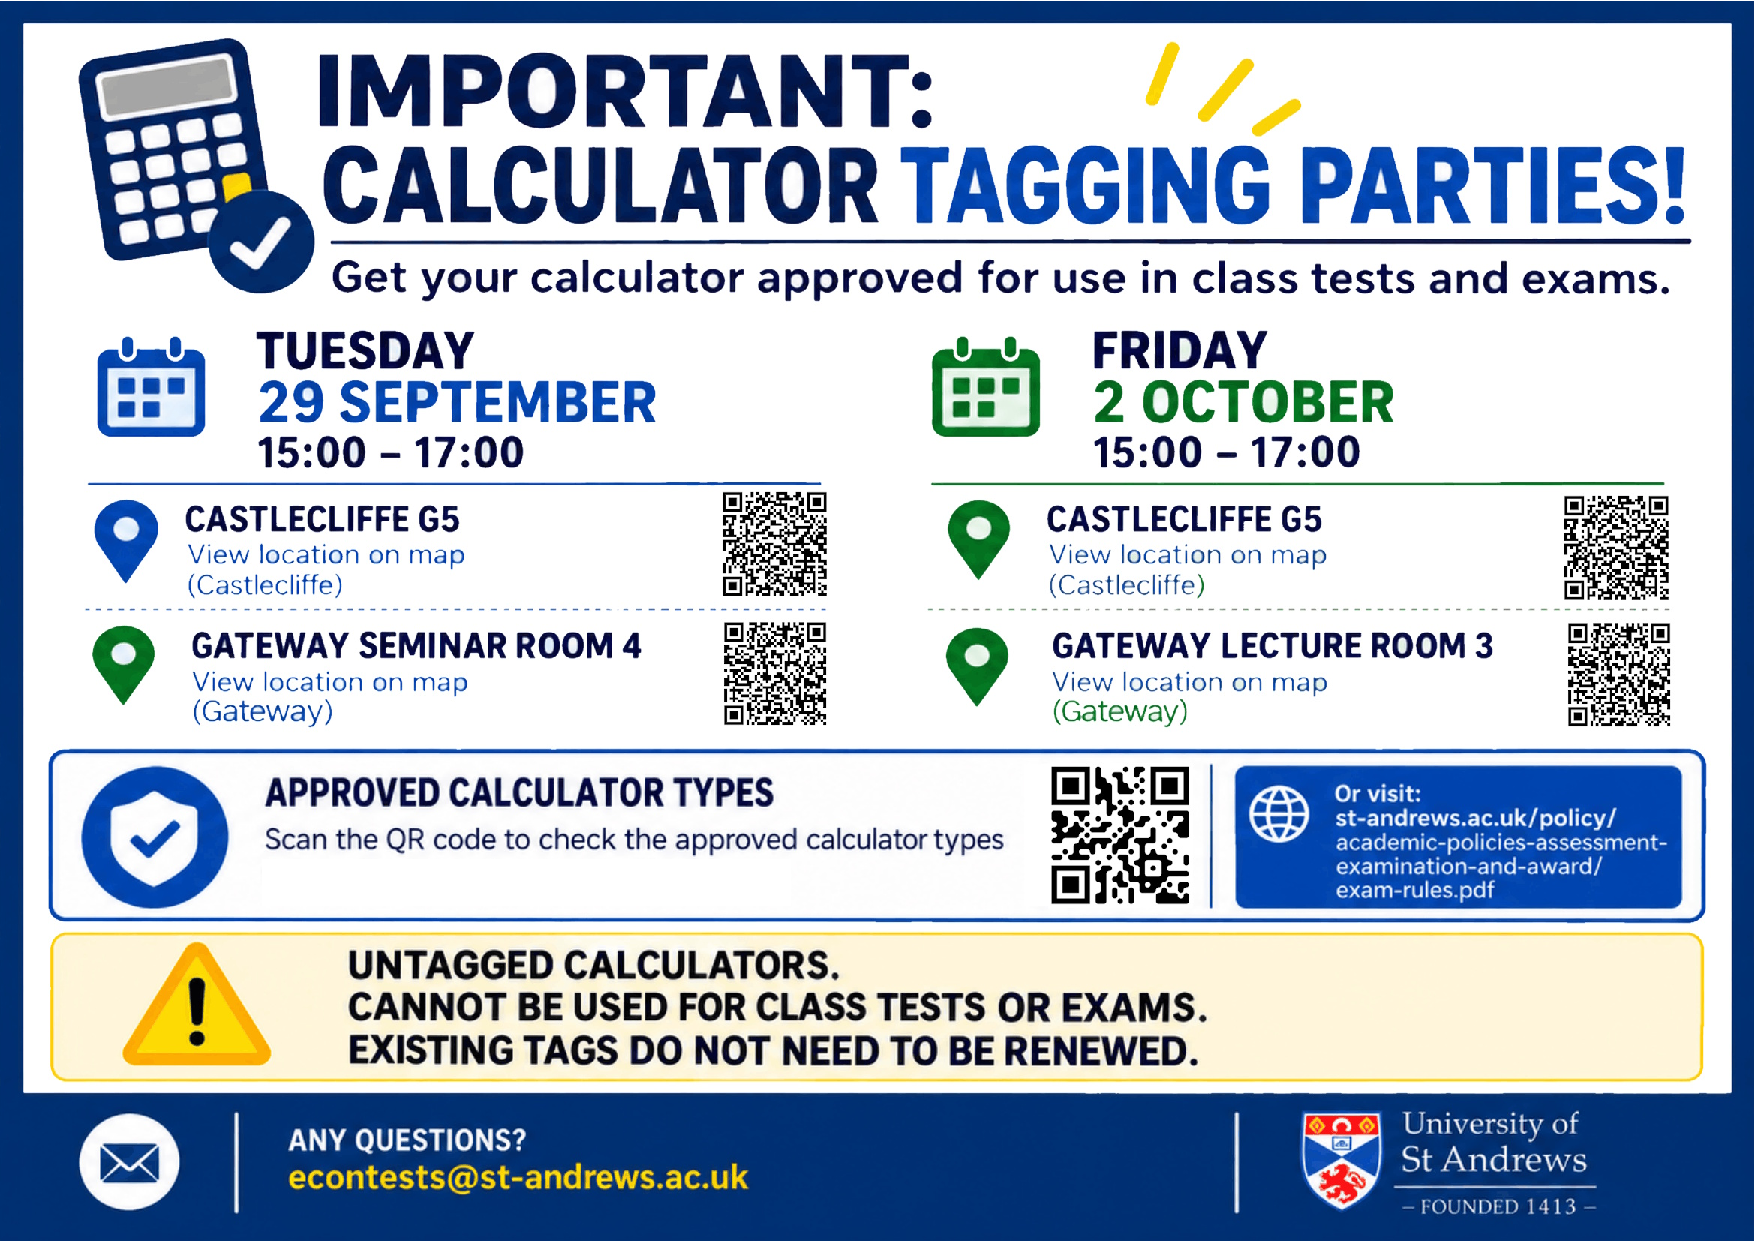
\includegraphics[
      width=\paperwidth,height=\paperheight,keepaspectratio
    ]{extra-slides/calculator tagging.pdf}};
  \end{tikzpicture}
\end{frame}
\begin{frame}[plain,noframenumbering]
  \begin{tikzpicture}[remember picture,overlay]
    \node[inner sep=0pt] at (current page.center) {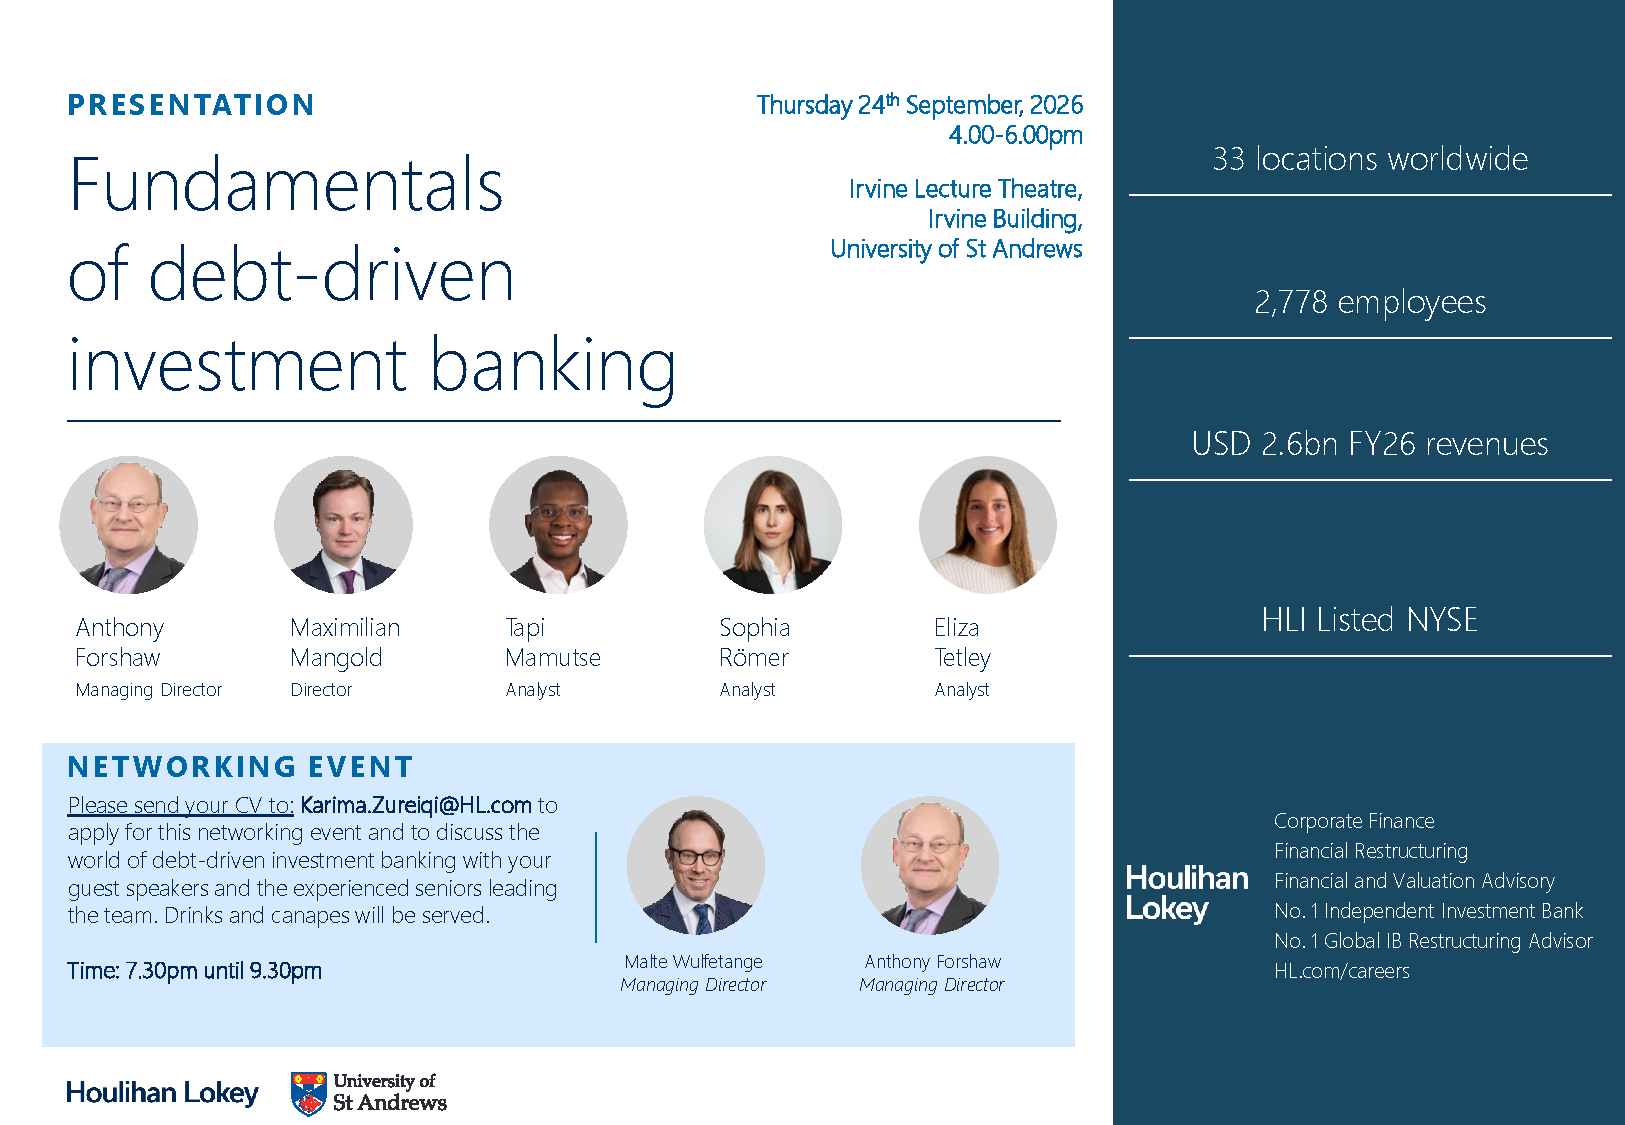
\includegraphics[
      width=\paperwidth,height=\paperheight,keepaspectratio
    ]{extra-slides/St Andrews Flyer - Houlihan Lokey - Sep-26.pdf}};
  \end{tikzpicture}
\end{frame}
\endgroup

\begin{frame}{Content of today's lecture}
\begin{columns}[t]
  \begin{column}{0.4\textwidth}
    \tableofcontents[sections={1}]
  \end{column}
  \begin{column}{0.4\textwidth}
    \tableofcontents[sections={2}]
  \end{column}
\end{columns}
\end{frame}


\begin{frame}
\frametitle{Reading}

\begin{enumerate}
  \item Brealey, R. A., Myers, S. C., Allen, F., \& Edmans, A. (2022). Principles of Corporate Finance (14th ed.). McGraw-Hill Education. ISBN: 978-1265074159. Chapters 7, 8, 9.

  \item Lundblad, C.\ (2007) The Risk Return Tradeoff in the Long Run: 1836--2003. 
        \emph{Journal of Financial Economics} 85, 123--150.\\
        \texttt{https://doi.org/10.1016/j.jfineco.2006.06.003}

  \item Bekaert, G., Hodrick, R.\,J., and Zhang, X.\ (2009) International Stock Return Comovements. 
        \emph{Journal of Finance} 64, 2591--2626.\\
        \texttt{https://doi.org/10.1111/j.1540-6261.2009.01512.x}


\item Fama, E.F., French, K.R. (2004) The Capital Asset Pricing Model: Theory and Evidence. \textit{Journal of Economic Perspectives} 18, 25-46.
\url{https://doi.org/10.1257/0895330042162430}


\item Graham, J.R., Harvey, C.R. (2001) The Theory and Practice of Corporate Finance: Evidence from the Field.  \textit{Journal of Financial Economics} 60, 187-243.
\url{https://doi.org/10.1016/S0304-405X(01)00044-7}
\end{enumerate}

\end{frame}


\section{Introduction to Risk and Return}




\subsection{Cost of Capital and Rate of Return}

\begin{frame}
\frametitle{\textnormal{Cost of Capital}}

\begin{itemize}

\item Corporate cost of capital is the return required by investors, which depends on the risk of the project

\item Another way to look at this: the estimated risk of a project [real assets] will determine how much investors would pay for a firm's securities [financial assets]

\item So one way to estimate the cost of capital is to estimate the expected return on securities of companies with similarly risky projects as those of your companies

\end{itemize}

\end{frame}

\begin{frame}
\frametitle{\textnormal{Rate of Return}}

\begin{itemize}
\item Return is a concept used to express the financial performance of an investment
\item Monetary return = (Amount received $-$ Amount invested)
\item Percentage return (Rate of return) = $ \frac{ \text{Monetary return}}{\text{Amount invested}}$


\vspace{6pt}
\textcolor{blue}{Example 1}

\vspace{6pt}
An investor pays £100 for a financial asset and receives £110 after a certain period.

Monetary return:		(110 $-$ 100) = £10

Percentage return:	$\frac{(110 \ - \ 100)}{100} = 10\%$

\end{itemize}

\end{frame}

\begin{frame}
\frametitle{\textnormal{Comparing Return for Different Holding Periods}}

\begin{itemize}
    \item In order to compare the returns on investments with different holding periods, we need to convert the rates of return for different holding periods into a common period.
\item Typically, all investment returns are expressed as an AER.
\item A rate of return of r for a holding period of n years can be converted to an AER using Eq.(1).

\end{itemize}
$$
    AER=(1+r)^{\frac{1}{n}}-1   \ (1)
    $$

\end{frame}

\begin{frame}
\frametitle{\textnormal{Annualized Rates of Returns}}

\textcolor{blue}{Example 2}

\vspace{6pt}
An investor compares returns of three investment opportunities. Which investment produces the highest rate of return?

\begin{table}
\begin{tabular}{l l l l}
\toprule
\text{Asset} & \text{Price(£)} & \text{Holding period} & \text{Expected receipt(£)} \\
\midrule
A & 97 & 6 months & 100 \\
B & 95 & 1 year & 100 \\
C & 25 & 20 years & 100 \\

    \bottomrule
    \end{tabular}
\end{table}

\begin{table}
\begin{tabular}{l l l l}

\toprule
\text{Asset} & \text{Rate of return} & \text{Annualized rate} & \text{} \\
\midrule
A & 3.09\% & 6.28\% & $=(1+0.0309)^{\frac{1}{0.5}}-1$ \\
B & 5.26\% & 5.26\% & $= (1 + 0.0526)^1 - 1$ \\
C & 300.00\% & 7.18\% & $= (1 + 3)^{\frac{1}{20}}-1$ \\
    \bottomrule
    \end{tabular}
\end{table}

\end{frame}

\subsection{Expected Returns and Risk}

\begin{frame}
\frametitle{\textnormal{Expected Rates of  Returns}}

\begin{itemize}
    \item The price of a financial asset tomorrow is uncertain, but beliefs about the market tomorrow could be quantified
\item How?
\begin{itemize}

\item [-]Historical rates of returns: the average of the realized returns for each period (year, quarter, month) during a particular historical time span

\item [-]Scenario and probability analysis: the expected (or mean) return is calculated as the weighted sum of the possible returns, where the weights correspond to the probabilities

\end{itemize}

\end{itemize}

\end{frame}

\begin{frame}
\frametitle{\textnormal{Expected Returns: Historical Data}}

$$
    \bar{r}=\frac{(r_1+r_2+\dots+r_T)}{T} =\frac{1}{T}\sum_{t=1}^T r_t  \ (2)
  $$

\begin{itemize}
    \item $\bar{r}$ = expected return of a security
\item $r_t$ = the realized return of a security in period t (month, quarter, year…)
\item T = the total number of periods during a historical time span

\end{itemize}

\end{frame}

\begin{frame}
\frametitle{\textnormal{Historical Data: Example}}

\textcolor{blue}{Example 3}
Calculate the expected monthly return on Barrick Gold's stock using price data below.

\begin{table}
\begin{tabular}{l l l}

\toprule
\text{Date} & {Price (\$)} & \text{Return(\%)} \\
\midrule
01/05/2015 &	11.79 &	\text{--}8.5\\
01/04/2015 &	12.89 &	18.8\\
02/03/2015 &	10.85 &	\text{--}15.8\\
02/02/2015 &	12.89 &	2.3\\
02/01/2015 &	12.6 & 18.9\\
01/12/2014 &	10.6 & \\
    \bottomrule
    \end{tabular}
\end{table}


\begin{center}
$$
\bar{r}_{ABX} = \frac{(\text{--}0.085+0.188-0.158+0.023+0.189)}{5}=\LBarrickMean\%
$$

\tiny {Source: Data from \url{https://uk.finance.yahoo.com}}
\end{center}
\end{frame}

\begin{frame}
\frametitle{\textnormal{Risk}}

\begin{itemize}
    \item Rates of returns (cost of capital) depend on the riskiness of a project, but how can risk be measured?
 \item Risk is the likelihood of deviations from the expected return
 \item One way to quantify risk is to estimate the variation of returns against the expected returns
 \item \textcolor{red}{Variance} is estimated by averaging squared deviations from the estimate of the expected return
 \item In practice, risk is measured by the \textcolor{red}{standard deviation}

\end{itemize}

\end{frame}

\begin{frame}
\frametitle{\textnormal{Graphical Presentation: Barrick Gold}}

\begin{center}
    \begin{tikzpicture}
\begin{axis}[lectureplot,width=11cm,height=5.1cm,xmin=.62,xmax=5.5,ymin=-27,ymax=27,
xtick={1,2,3,4,5},xticklabels={Jan 2015,Feb 2015,Mar 2015,Apr 2015,May 2015},
ytick={-20,-10,0,10,20},yticklabel={\pgfmathprintnumber{\tick}\%},
xlabel={Month},ylabel={Monthly return}]
\addplot[black!35,thin] coordinates {(.62,0)(5.5,0)};
\addplot[StAndrewsMidGreen,thick] coordinates {(.62,\LBarrickMean)(5.5,\LBarrickMean)};
\addplot[StAndrewsRed,dashed,thin] coordinates {(1,\LBarrickMean)(1,18.87)};
\addplot[StAndrewsRed,dashed,thin] coordinates {(3,\LBarrickMean)(3,-15.83)};
\addplot[StAndrewsBlue,mark=*,mark size=1.7pt,smooth] table[x=t,y=ret]{generated/barrick.dat};
\node[anchor=south,font=\footnotesize,text=StAndrewsMidGreen,yshift=3pt] at (axis cs:2.8,\LBarrickMean) {Mean $=\LBarrickMean\%$};
\draw[-{Stealth[length=4pt]},StAndrewsRed] (axis cs:1.32,22.5) -- (axis cs:1.04,12.5);
\node[anchor=west,font=\footnotesize,text=StAndrewsRed] at (axis cs:1.37,23.5) {Deviation $=0.189-0.031$};
\draw[-{Stealth[length=4pt]},StAndrewsRed] (axis cs:3.5,-21) -- (axis cs:3.04,-7.5);
\node[anchor=east,font=\footnotesize,text=StAndrewsRed] at (axis cs:5.45,-23) {Deviation $=-0.158-0.031$};
\node[anchor=south,font=\footnotesize] at (axis cs:1,19.4) {18.9\%};
\node[anchor=north east,font=\footnotesize,xshift=-3pt,yshift=-3pt] at (axis cs:2,2.3) {2.3\%};
\node[anchor=north,font=\footnotesize,yshift=-3pt] at (axis cs:3,-15.83) {$-15.8\%$};
\node[anchor=south,font=\footnotesize] at (axis cs:4,19.3) {18.8\%};
\node[anchor=north,font=\footnotesize,yshift=-4pt] at (axis cs:5,-8.53) {$-8.5\%$};
\end{axis}\end{tikzpicture}

    \\
    \tiny {Source: Author's own calculation using stock data from \url{https://uk.finance.yahoo.com  }
}

\end{center}

\end{frame}

\begin{frame}
\frametitle{\textnormal{Measure of Risk: Historical Data}}

$$
\text {Variance} = \sigma^2 = \frac{1}{(T-1)} \sum_{t=1}^{T} (r_t-\bar{r})^2 \ (4a)$$

$$
\text {Standard Deviation} = \sigma = \sqrt{\sigma^2} \ (4b) 
$$

\textcolor{red}{\underline{Back to Example 3:}}

\centering{$\bar{r} = \LBarrickMean\%$}

\vspace{-8pt}
\begin{table}
\begin{tabular}{l l l l l}

\toprule
\text{Date}& \text{Return (\%)}&	\text{Variance} \\
\midrule
01/05/2015	&\text {--}8.5 &$(\text{--} 0.085-0.031)^2$=0.01356	\\
01/04/2015	&18.8	& $(0.188-0.031)^2$=0.02456	\\
02/03/2015	&\text{--}15.8 & $(\text{--} 0.158-0.031)^2$=0.03590	\\
02/02/2015	&2.3	& $(0.023-0.031)^2$=0.00007	\\
02/01/2015 & 18.9&	$(0.189-0.031)^2$=0.02483 \\
    \bottomrule
    \end{tabular}
\end{table}

\vspace{-8pt}
\centering{$\sigma^2 = \LBarrickVar, \sigma = \LBarrickSD\%$}

\end{frame}

\begin{frame}
\frametitle{\textnormal{Probability Distribution}}

\begin{itemize}
    \item Probabilities are assigned to different expected outcomes in order to estimate the \textcolor{blue}{mean} and \textcolor{red}{variance}
\item If all possible events are listed and a probability is assigned to each event, the listing is called probability distribution
\item Probability distribution of returns can be approximated by a bell-shaped curve known as normal distribution

\end{itemize}
\end{frame}

\begin{frame}
\frametitle{\textnormal{Probability Ranges for a Normal Distribution}}

\begin{center}

\begin{tikzpicture}
\begin{axis}[lectureplot,width=11.4cm,height=5.4cm,xmin=-58,xmax=83,ymin=0,ymax=1.3,
axis lines=middle,axis y line=none,
xtick={\LNormalA,\LNormalB,\LNormalC,\LNormalD,\LNormalE,\LNormalF,\LNormalG},
xticklabels={{$-3\sigma$\\$\LNormalA\%$},{$-2\sigma$\\$\LNormalB\%$},{$-1\sigma$\\$\LNormalC\%$},
             {$\LNormalD\%$},{$+1\sigma$\\$\LNormalE\%$},{$+2\sigma$\\$\LNormalF\%$},{$+3\sigma$\\$\LNormalG\%$}},
xticklabel style={font=\scriptsize,align=center,yshift=-1pt},
xlabel={Return on stocks},xlabel style={at={(axis description cs:0.5,0)},anchor=north,yshift=-27pt}]
\addplot[draw=none,name path=base] coordinates {(-58,0)(83,0)};
\addplot[StAndrewsBurgundy!55,name path=bell,smooth] table[x=x,y=density]{generated/normal.dat};
\addplot[StAndrewsBurgundy!20] fill between[of=bell and base];
\addplot[black!55,dashed,thin] coordinates {(\LNormalC,0)(\LNormalC,.62)(\LNormalE,.62)(\LNormalE,0)};
\addplot[black!55,dashed,thin] coordinates {(\LNormalB,0)(\LNormalB,.34)(\LNormalF,.34)(\LNormalF,0)};
\addplot[black!55,dashed,thin] coordinates {(\LNormalA,0)(\LNormalA,.13)(\LNormalG,.13)(\LNormalG,0)};
\node[anchor=south,font=\footnotesize] at (axis cs:\LNormalD,.645) {68.26\%};
\node[anchor=south,font=\footnotesize] at (axis cs:\LNormalD,.365) {95.44\%};
\node[anchor=south,font=\footnotesize] at (axis cs:\LNormalD,.155) {99.74\%};
\node[anchor=north west,font=\small] at (axis cs:-58,1.3) {Probability};
\end{axis}\end{tikzpicture}

    \\

    $\bar{r} = 12.3\%$ and $\sigma = 20.2\%$
    \\
    \vspace{6pt}
        \tiny {Source: Hillier, Ross, Westerfield, Jaffe \& Jordan (2016) Corporate Finance 3rd ed. (Figure 9.7, page 242).}
\end{center}

\end{frame}

\subsection{Portfolio Theory and Diversification}

\begin{frame}
\frametitle{\textnormal{Diversification}}

\begin{itemize}

\item Diversification can substantially reduce risk (the variability of returns) without an equivalent reduction in expected returns
\item This reduction in risk arises because worse-than-expected returns from one asset are offset by better-than-expected returns from another
\item So it is less risky to hold \textcolor{red}{a portfolio of investments} rather than relying on a single investment

\end{itemize}

\end{frame}

\begin{frame}
\frametitle{\textnormal{Portfolio Theory}}

\begin{columns}

\column{0.5\textwidth}

\begin{itemize}
    \item Portfolio theory was first developed by Harry Markowitz in 1952
\item Markowitz gave us the tools for identifying portfolios which give the highest return for a particular level of risk (depending on personal risk aversion of investors)
\end{itemize}

\column{0.5\textwidth}
\begin{center}

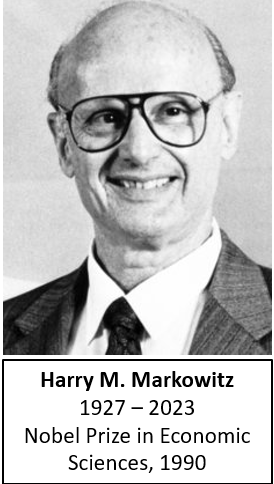
\includegraphics[scale=0.40]{HM.png}
\end{center}

\end{columns}

\end{frame}

\begin{frame}
\frametitle{\textnormal{Portfolio Returns}}

\begin{itemize}
    \item The expected return of a portfolio is the weighted sum of the expected returns of the individual assets in the portfolio
\end{itemize}

$$
\bar{r}_p = w_1 \bar{r}_1 + w_2 \bar{r}_2+\dots+w_N \bar{r}_N = \sum_{i=1}^{N} w_i \bar{r}_i  \ (6) $$

\begin{itemize}
    \item $\bar{r}_p$ = expected return of a portfolio
\item $w_i$ = the proportion of value invested in security i
\item $w_1+w_2+\dots+w_n=1$ \textcolor{red}{(weights can be negative)}
\item $\bar{r}_i$ = expected return of security i
\item N = the total number of securities in the portfolio

\end{itemize}

\end{frame}

\begin{frame}
\frametitle{\textnormal{Portfolio Returns: Example 4}}

Suppose you want to purchase stocks of Wal-Mart (WMT) and Honeywell (HON) listed on NYSE. You have estimated the monthly rates of returns on these two stocks as shown below.

\begin{table}
\begin{tabular}{l l l}

\toprule
\text{Date}&	\text{Wal-Mart} &\text{Honeywell} \\
\midrule
04/01/2016&	0.00261&	\text{--}0.00966\\
01/12/2015&	0.05053	&\text{--}0.00366\\
02/11/2015&	0.02795	&0.01234\\
01/10/2015&	\text{--}0.11721&	0.09072\\
01/09/2015	&0.0017	&\text{--}0.04614\\
    \bottomrule
    \end{tabular}
\end{table}
\begin{center}
\tiny {Source: Data from \url{https://uk.finance.yahoo.com}}
\end{center}

You intend to invest 10\% of your money in WMT and 90\% in HON. Calculate the expected return of a portfolio of these two stocks.

\end{frame}

\begin{frame}
\frametitle{\textnormal{Portfolio Returns: Solution}}

\textcolor{blue}{Example 4: Solution}
\\

$$\bar{r}_{WMT} = \frac{1}{T} \sum_{t=1}^{T} r_t = \text{--}0.688\%
$$

$$\bar{r}_{HON} = 0.872\%$$

$$
\bar{r}_{(WMT+HON)} = w_{WMT} \times \bar{r}_{WMT} + w_{HON} \times \bar{r}_{HON} =
$$
$$
=0.1 \times (\text{--}0.00688)+0.9 \times 0.00872=0.716\%
$$

\end{frame}

\begin{frame}
\frametitle{\textnormal{Portfolio Risk: Formula}}

\begin{itemize}
    \item Portfolio risk is reflected by the covariance: the extent to which returns on two assets 'move together'
\item The standard deviation for a portfolio of N assets:

$$   \sigma_p = \sqrt{\sum_{i=1}^{N} \sum_{j=1}^{N} w_i w_j \sigma_{ij}  }  \ (7) $$

\item $\sigma_{ij}$ = covariance between returns on assets \textit{i} and \textit{j}

\end{itemize}

\end{frame}

\begin{frame}
\frametitle{\textnormal{Covariance and Correlation}}

\begin{itemize}
\item Covariance:
$$    \sigma_{ij}=\sum_{s=1}^{S}[(r_{s,i}- \bar{r}_i)(r_{s,j}-\bar{r}_j)] p_s \ (8)$$

$$    \sigma_{ij}=\frac{1}{(T-1)} \sum_{t=1}^{T}(r_{t,i}-\bar{r}_i)(r_{t,j}-\bar{r}_j) \ (9) $$


\item Correlation coefficient:

$$
    \rho_{ij}=\frac{\sigma_{ij}}{(\sigma_i \times \sigma_j)} \ (10) $$

\item Correlation coefficient is always between \text{--}100\% and +100\%

\end{itemize}

\end{frame}

\begin{frame}
\frametitle{\textnormal{Portfolio Risk: Example}}

\textcolor{red}{\underline{Back to Example 4:}}
\\
\vspace{6pt}
Calculate the variance and standard deviation of your portfolio.
\\
The variance of a two-asset portfolio = the square-weighted sum of the variances plus twice the cross-weighted covariance (Eq.7):
\\
\vspace{-4pt}
\begin{align}
    \sigma_{p(2)}^2= w_1 w_1 \sigma_{11} + w_1 w_2 \sigma_{12} + w_2 w_1 \sigma_{21} + w_2 w_2 \sigma_{22} \\
= w_1^2 \sigma_1^2+w_2^2 \sigma_2^2+2w_1 w_2 \sigma_{12} = w_1^2 \sigma_1^2+w_2^2 \sigma_2^2+2w_1 w_2 \sigma_1 \sigma_2 \rho_{12}   
\end{align}
\vspace{-2pt}
\text {We need to calculate:}

\vspace{6pt}
\setlength{\parindent}{0.5cm}
(1) $\sigma_{WMT}^2$ and $\sigma_{HON}^2$ (Eq.4a)

\vspace{6pt}
(2) $\sigma_{(WMT,HON)}$ (Eq.9)

\end{frame}

\begin{frame}
\frametitle{\textnormal{Portfolio Risk: Solution}}

\textcolor{red}{\underline{Back to Example 4:}}
\\
\vspace{6pt}
$
\sigma_{WMT}^2 = 0.00421 \text{ and } \sigma_{HON}^2=0.00256   $
\\
$$\sigma_{(WMT,HON)}= \frac{[0.00261 - (\text{--}0.00688)] \times [(\text{--}0.00966)-0.00872]}{(5-1)}
$$
$$ + \frac{[0.05053 - (\text{--}0.00688)] \times [(\text{--}0.00366)- 0.00872]}{(5 - 1)}$$
$$+ \frac{[0.02795 - (\text{--}0.00688)] \times [0.01234 - 0.00872]}{(5 - 1)}$$
$$+ \frac{[(\text{--}0.11721) - (\text{--}0.00688)] \times [0.09072 - 0.00872]}{(5 - 1)}$$
$$+ \frac {[0.00170 - (\text{--}0.00688)] \times [(\text{--}0.04614) - 0.00872]}{(5 - 1)}=\text{--}0.00257$$
\\
$\sigma_{(WMT+HON)}^2=0.00165 \text{ and } \sigma_{(WMT+HON)}=0.04065=4.07\% \text{(monthly)} $

\end{frame}

\subsection{Efficient Frontier and Portfolio Optimization}

\begin{frame}
\frametitle{\textnormal{The Opportunity Set: Individual Stocks}}

\begin{center}

    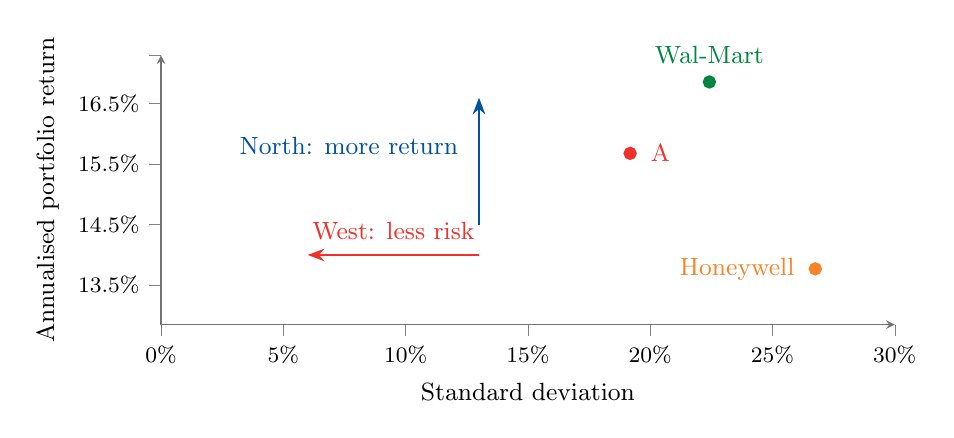
\begin{tikzpicture}
\begin{axis}[frontierplot]
\addplot[only marks,mark=*,mark size=2pt,StAndrewsMidGreen] coordinates {(\LSDWmt,\LMeanWmt)};
\addplot[only marks,mark=*,mark size=2pt,StAndrewsOrange] coordinates {(\LSDHon,\LMeanHon)};
\addplot[only marks,mark=*,mark size=2pt,StAndrewsRed] coordinates {(\LSDTwoMV,\LMeanTwoMV)};
\node[anchor=south,font=\small,text=StAndrewsMidGreen,yshift=3pt] at (axis cs:\LSDWmt,\LMeanWmt) {Wal-Mart};
\node[anchor=east,font=\small,text=StAndrewsOrange,xshift=-4pt] at (axis cs:\LSDHon,\LMeanHon) {Honeywell};
\node[anchor=west,font=\small,text=StAndrewsRed,xshift=4pt] at (axis cs:\LSDTwoMV,\LMeanTwoMV) {A};
\draw[-{Stealth[length=6pt]},StAndrewsBlue,thick] (axis cs:13,14.5) -- (axis cs:13,16.6);
\draw[-{Stealth[length=6pt]},StAndrewsRed,thick] (axis cs:13,14.0) -- (axis cs:6,14.0);
\node[anchor=east,font=\small,text=StAndrewsBlue,xshift=-4pt] at (axis cs:13,15.8) {North: more return};
\node[anchor=south,font=\small,text=StAndrewsRed,yshift=2pt] at (axis cs:9.5,14.0) {West: less risk};
\end{axis}\end{tikzpicture}


    \tiny {Source: Author's own calculation using monthly stock prices from \LWindowFrom--\LWindowTo, available at \url{https://uk.finance.yahoo.com}  }
\end{center}
\end{frame}

\begin{frame}
\frametitle{\textnormal{The Opportunity Set: Portfolios}}

\begin{center}

    \begin{tikzpicture}
\begin{axis}[frontierplot]
\addplot[StAndrewsOrange,thick] table[x expr=100*\thisrow{sd},y expr=100*\thisrow{ret}]{generated/two_stock.dat};
\addplot[only marks,mark=*,mark size=2pt,StAndrewsMidGreen] coordinates {(\LSDWmt,\LMeanWmt)};
\addplot[only marks,mark=*,mark size=2pt,StAndrewsOrange] coordinates {(\LSDHon,\LMeanHon)};
\addplot[only marks,mark=*,mark size=2pt,StAndrewsRed] coordinates {(\LSDTwoOpt,\LMeanTwoOpt)};
\addplot[only marks,mark=*,mark size=2pt,StAndrewsBlue] coordinates {(\LSDTwoMV,\LMeanTwoMV)};
\node[anchor=south east,font=\small,text=StAndrewsMidGreen,yshift=2pt] at (axis cs:\LSDWmt,\LMeanWmt) {Wal-Mart (100\%; 0\%)};
\node[anchor=north east,font=\small,text=StAndrewsOrange,yshift=-2pt] at (axis cs:\LSDHon,\LMeanHon) {Honeywell (0\%; 100\%)};
\node[anchor=south east,font=\footnotesize,text=StAndrewsRed,xshift=-4pt,yshift=2pt] at (axis cs:\LSDTwoOpt,\LMeanTwoOpt) {Optimal (\LTwoOptwmt\%; \LTwoOpthon\%)};
\node[anchor=north east,font=\footnotesize,text=StAndrewsBlue,xshift=-4pt,yshift=-2pt] at (axis cs:\LSDTwoMV,\LMeanTwoMV) {Minimum variance (\LTwoMVwmt\%; \LTwoMVhon\%)};
\node[anchor=west,font=\small,text=StAndrewsBurgundy,align=left] at (axis cs:.8,14.6)
 {Two-stock frontier\\[3pt] Correlation $=\LTwoCorr$};
\end{axis}\end{tikzpicture}


    \tiny {Source: Author's own calculation using monthly stock prices from \LWindowFrom--\LWindowTo, available at \url{https://uk.finance.yahoo.com  }}
\end{center}

\end{frame}

\begin{frame}
\frametitle{\textnormal{The Opportunity Set: Interpretations}}

\begin{itemize}
    \item The curved line connecting different portfolios when the weights are changed represents an opportunity set or feasible set of portfolios for an investor
 \item An investor cannot achieve any point above (below) the curve because s/he cannot increase (reduce) the returns on the individual securities, reduce (increase) the standard deviations of the securities, or reduce (increase) the correlations between securities
 \item The \textcolor{blue}{minimum-variance} portfolio is the one with the lowest risk while the \textcolor{red}{optimal} portfolio is the one that has the highest return per unit of risk

\end{itemize}
\end{frame}

\begin{frame}
\frametitle{\textnormal{The Efficient Frontier}}

\begin{itemize}
    \item The section of the opportunity set above the minimum variance portfolio is the efficient frontier
\item The efficient portfolios are those which lie on the efficient frontier and offer the highest return for a given level of risk: there is no way to reduce the risk of the efficient portfolio without a decrease in its expected return
\item The optimal portfolio is the one that has the highest return per unit of risk

\end{itemize}

\end{frame}

\begin{frame}
\frametitle{\textnormal{The Opportunity Set: Short Sale}}

\begin{center}
    \begin{tikzpicture}
\begin{axis}[frontierplot,xmax=40,ymax=18.6,ytick={13.5,14.5,15.5,16.5,17.5,18.6},
yticklabels={13.5\%,14.5\%,15.5\%,16.5\%,17.5\%,{}},xtick={0,5,10,15,20,25,30,35,40}]
\addplot[StAndrewsOrange,thick] table[x expr=100*\thisrow{sd},y expr=100*\thisrow{ret}]{generated/two_stock.dat};
\addplot[StAndrewsOrange,thick,dotted] table[x expr=100*\thisrow{sd},y expr=100*\thisrow{ret}]{generated/two_short.dat};
\addplot[only marks,mark=*,mark size=2pt,StAndrewsMidGreen] coordinates {(\LSDWmt,\LMeanWmt)};
\addplot[only marks,mark=*,mark size=2pt,StAndrewsOrange] coordinates {(\LSDHon,\LMeanHon)};
\addplot[only marks,mark=*,mark size=1.8pt,StAndrewsBlue] table[x expr=100*\thisrow{sd},y expr=100*\thisrow{ret}]{generated/two_short_marks.dat};
\addplot[only marks,mark=*,mark size=2pt,StAndrewsRed] coordinates {(\LSDTwoOpt,\LMeanTwoOpt)};
\node[anchor=north west,font=\small,text=StAndrewsMidGreen,xshift=3pt,yshift=-2pt] at (axis cs:\LSDWmt,\LMeanWmt) {Wal-Mart (100\%; 0\%)};
\node[anchor=south west,font=\small,text=StAndrewsOrange,xshift=2pt,yshift=2pt] at (axis cs:\LSDHon,\LMeanHon) {Honeywell (0\%; 100\%)};
\node[anchor=south east,font=\footnotesize,text=StAndrewsRed,xshift=-4pt,yshift=2pt] at (axis cs:\LSDTwoOpt,\LMeanTwoOpt) {Optimal (\LTwoOptwmt\%; \LTwoOpthon\%)};
\node[anchor=south east,font=\footnotesize,text=StAndrewsBlue,yshift=2pt] at (axis cs:\LSDShortA,\LMeanShortA) {(\LShortWA\%; $\LShortHA$\%)};
\node[anchor=south east,font=\footnotesize,text=StAndrewsBlue,yshift=2pt] at (axis cs:\LSDShortB,\LMeanShortB) {(\LShortWB\%; $\LShortHB$\%)};
\node[anchor=west,font=\small,text=StAndrewsBurgundy,align=left] at (axis cs:.8,14.6)
 {Short sales allowed:\\[3pt] weights beyond 100\%};
\end{axis}\end{tikzpicture}


    \tiny {Source: Author's own calculation using monthly stock prices from \LWindowFrom--\LWindowTo, available at \url{https://uk.finance.yahoo.com  }}

\end{center}

\end{frame}

\begin{frame}
\frametitle{\textnormal{The Opportunity Set: Adding More Stocks}}

\begin{center}
    \begin{tikzpicture}
\begin{axis}[frontierplot]
\addplot[StAndrewsBlue,thick] table[x expr=100*\thisrow{sd},y expr=100*\thisrow{ret}]{generated/five_stock.dat};
\addplot[only marks,mark=*,mark size=1.6pt,black] table[x expr=100*\thisrow{sd},y expr=100*\thisrow{ret}]{generated/five_inframe.dat};
\addplot[only marks,mark=*,mark size=2pt,StAndrewsRed] coordinates {(\LSDFiveOpt,\LMeanFiveOpt)};
\node[anchor=west,font=\small,xshift=3pt] at (axis cs:\LSDWmt,\LMeanWmt) {Wal-Mart};
\node[anchor=west,font=\small,xshift=3pt] at (axis cs:\LSDKo,\LMeanKo) {Coca-Cola};
\node[anchor=west,font=\small,xshift=3pt] at (axis cs:\LSDHon,\LMeanHon) {Honeywell};
\node[anchor=south east,font=\footnotesize,text=StAndrewsRed,xshift=-4pt,yshift=3pt] at (axis cs:\LSDFiveOpt,\LMeanFiveOpt) {Optimal};
\node[anchor=north east,font=\footnotesize,text=StAndrewsBlue,xshift=-4pt,yshift=-3pt] at (axis cs:\LSDFiveMV,\LMeanFiveMV) {Minimum variance};
\node[anchor=north west,font=\small,text=StAndrewsBurgundy,align=left] at (axis cs:.8,15.0)
 {Five-stock frontier:\\[2pt] Agnico Eagle, Citigroup,\\[2pt] Coca-Cola, Honeywell, Wal-Mart};
\end{axis}\end{tikzpicture}


    \tiny {Source: Author's own calculation using monthly stock prices from \LWindowFrom--\LWindowTo, available at \url{https://uk.finance.yahoo.com  }}

\end{center}

\end{frame}

\begin{frame}
\frametitle{\textnormal{Two-Stock vs. Five-Stock Portfolio}}

\begin{center}
    \begin{tikzpicture}
\begin{axis}[frontierplot]
\addplot[StAndrewsOrange,thick] table[x expr=100*\thisrow{sd},y expr=100*\thisrow{ret}]{generated/two_stock.dat};
\addplot[StAndrewsBlue,thick] table[x expr=100*\thisrow{sd},y expr=100*\thisrow{ret}]{generated/five_stock.dat};
\addplot[only marks,mark=*,mark size=1.6pt,black] table[x expr=100*\thisrow{sd},y expr=100*\thisrow{ret}]{generated/five_inframe.dat};
\addplot[only marks,mark=*,mark size=2pt,StAndrewsRed] coordinates {(\LSDFiveOpt,\LMeanFiveOpt)};
\node[anchor=west,font=\small,xshift=3pt] at (axis cs:\LSDWmt,\LMeanWmt) {Wal-Mart};
\node[anchor=west,font=\small,xshift=3pt] at (axis cs:\LSDHon,\LMeanHon) {Honeywell};
\node[anchor=south east,font=\footnotesize,text=StAndrewsRed,xshift=-4pt,yshift=3pt] at (axis cs:\LSDFiveOpt,\LMeanFiveOpt) {Optimal};
\node[anchor=north east,font=\footnotesize,text=StAndrewsBlue,xshift=-4pt,yshift=-3pt] at (axis cs:\LSDFiveMV,\LMeanFiveMV) {Minimum variance};
\node[anchor=north west,font=\small,text=StAndrewsOrange] at (axis cs:.8,16.6) {Two-stock frontier};
\node[anchor=north west,font=\small,text=StAndrewsBlue] at (axis cs:.8,17.25) {Five-stock frontier};
\end{axis}\end{tikzpicture}


    \tiny {Source: Author's own calculation using monthly stock prices from \LWindowFrom--\LWindowTo, available at \url{https://uk.finance.yahoo.com  }}

\end{center}

\end{frame}

\begin{frame}
\frametitle{\textnormal{The Effect of Correlation}}

\begin{center}
    \begin{tikzpicture}
\begin{axis}[frontierplot,ymin=11.6]
\addplot[StAndrewsBlue!35,thick] table[x expr=100*\thisrow{sd},y expr=100*\thisrow{ret}]{generated/corr_minus.dat};
\addplot[StAndrewsBlue,thick] table[x expr=100*\thisrow{sd},y expr=100*\thisrow{ret}]{generated/corr_mid.dat};
\addplot[StAndrewsOrange,thick] table[x expr=100*\thisrow{sd},y expr=100*\thisrow{ret}]{generated/two_stock.dat};
\addplot[StAndrewsRed,thick] table[x expr=100*\thisrow{sd},y expr=100*\thisrow{ret}]{generated/corr_plus.dat};
\addplot[only marks,mark=*,mark size=2pt,StAndrewsMidGreen] coordinates {(\LSDWmt,\LMeanWmt)};
\addplot[only marks,mark=*,mark size=2pt,StAndrewsOrange] coordinates {(\LSDHon,\LMeanHon)};
\node[anchor=south east,font=\small,text=StAndrewsMidGreen,yshift=2pt] at (axis cs:\LSDWmt,\LMeanWmt) {Wal-Mart};
\node[anchor=north west,font=\small,text=StAndrewsOrange,xshift=2pt] at (axis cs:\LSDHon,\LMeanHon) {Honeywell};
\node[anchor=north west,font=\footnotesize,align=left,inner sep=1pt] at (axis cs:.8,14.3)
 {\textcolor{StAndrewsBlue!60}{$\rho=-1$\quad risk removed completely}\\[3pt]
  \textcolor{StAndrewsBlue}{$\rho=-0.7$}\\[3pt]
  \textcolor{StAndrewsOrange}{$\rho=\LTwoCorr$\quad (actual)}\\[3pt]
  \textcolor{StAndrewsRed}{$\rho=+1$\quad no diversification}};
\end{axis}\end{tikzpicture}


    \tiny {Source: Author's own calculation using monthly stock prices from \LWindowFrom--\LWindowTo, available at \url{https://uk.finance.yahoo.com}}
\end{center}
\end{frame}

\subsection{Limits of Diversification}

\begin{frame}
\frametitle{\textnormal{The Limit of Diversification}}

\begin{itemize}
\item There are risk factors that affect a large number of stocks in a similar way
\item These risk factors could not be reduced through diversification even when holding a portfolio which includes all stocks in the market
\item Such factors as changes in GDP, inflation, interest rate…
\item They are known as non-diversifiable or market risk or systematic risks
\item \textcolor{green}{Total risk} = \textcolor{blue}{firm-specific risk} + \textcolor{red}{market risk}

\end{itemize}

\end{frame}

\begin{frame}
\frametitle{\textnormal{Graphical Presentation}}

\begin{center}

\begin{tikzpicture}
\begin{axis}[lectureplot,width=9.6cm,height=4.9cm,xmin=0,xmax=31,ymin=0,ymax=.125,
xtick={1,5,10,15,20,25,30},ytick={\LDivFloor,\LDivVar},yticklabels={$\overline{\text{cov}}$,$\overline{\text{var}}$},
xlabel={Number of securities},ylabel={Variance of the portfolio's return}]
\addplot[black!45,dashed,thin] coordinates {(0,\LDivFloor)(31,\LDivFloor)};
\addplot[StAndrewsBurgundy,thick] table[x=n,y=variance]{generated/diversification.dat};
\draw[-{Stealth[length=5pt]},black!70] (axis cs:5.5,.1) -- (axis cs:2.3,.076);
\node[anchor=west,font=\footnotesize,align=left] at (axis cs:5.8,.1)
 {Diversifiable, unique\\ or unsystematic risk};
\draw[-{Stealth[length=5pt]},black!70] (axis cs:13,.035) -- (axis cs:13,.0175);
\node[anchor=south,font=\footnotesize,align=center] at (axis cs:13,.0375)
 {Portfolio, market or systematic risk};
\end{axis}\end{tikzpicture}


\tiny {Source: Hillier, Ross, Westerfield, Jaffe and Jordan (2021) \textit{Corporate Finance} 3rd ed. (Figure 10.7, page 272)}
\end{center}
\end{frame}

\section{CML, SML and the CAPM}

\subsection{Risk-Free Asset and Portfolio Combinations}

\begin{frame}



\frametitle{\textnormal{Topics Covered}}

\begin{itemize}

\item One Risk-Free Asset and a Risky Portfolio 
\item CML \& SML
\item CAPM
\item Risk in a Context of Fully Diversified Portfolio
\item Cost of Equity
\item Criticisms of CAPM and Its Use in Practice


\end{itemize}

\end{frame}

%----------------------------------------------
%                    SLIDE 3
%----------------------------------------------



%----------------------------------------------
%                    SLIDE 4
%----------------------------------------------

\begin{frame}

\frametitle{\textnormal{Portfolio of a Risky Portfolio \&  a Riskless Asset}}

\begin{itemize}

\item An investor could combine a risky portfolio (assets in this portfolio are all risky) with an investment in a risk-free security
\item Back to the 5-security portfolio: AEM, WMT, HON, C and KO
\item What is the return and risk of the portfolio of a five-risky-asset portfolio and a risk-free security?
\item What does the opportunity set look like?
\item Is the efficient frontier better?



 

\end{itemize}


\end{frame}


%----------------------------------------------
%                    SLIDE 5
%----------------------------------------------
\begin{frame}

\frametitle{\textnormal{The Return and Risk}}
Let
\begin{itemize}
\item $w_1$ = the amount of money invested in the risk-free asset
\item $w_2$ = the amount of money invested in the risky portfolio
\item $r_f$ = the return on the risk-free asset = constant
\item $r_2$ = the return on the risky portfolio
\item $\sigma_2$ = the standard deviation of the risky portfolio
\end{itemize}
The expected return and standard deviation of the portfolio including the risky portfolio and risk-free asset:
\setlength{\parindent}{0.5cm}
\begin{itemize}
    \item $\bar{r}_p = w_1 r_f + w_2 \bar{r}_2$
    \item $\sigma_p^2 = w_1^2 \sigma_f^2 + w_2^2 \sigma_2^2+2w_1 w_2 \sigma_{f,2}$
    \item $\sigma_f^2=0 \text{ and}  \ \sigma_{f,2}=0$
    \item $\sigma_p =w_2 \sigma_2$
\end{itemize}
\end{frame}

%----------------------------------------------
%                    SLIDE 6
%----------------------------------------------
\begin{frame}

\frametitle{\textnormal{Characteristics of the Portfolio}}

\begin{itemize}
    \item The standard deviation is only a fraction of the risky portfolio, based on the amount we invest in it
\item As we increase the amount invested in the risky portfolio, we increase both risk and return proportionally 
\item This combination is a straight line connecting the risky point and the risk-free one

\end{itemize}


\end{frame}


%----------------------------------------------
%                    SLIDE 7
%----------------------------------------------
\begin{frame}

\frametitle{\textnormal{The Risk-Return Combinations}}

\begin{center}
    
    \begin{tikzpicture}
\begin{axis}[lectureplot,width=10.9cm,height=5cm,xmin=0,xmax=35,ymin=3,ymax=24,
xtick={0,5,10,15,20,25,30,35},ytick={4,9,14,19,24},
xticklabel={\pgfmathprintnumber{\tick}\%},yticklabel={\pgfmathprintnumber{\tick}\%},
xlabel={Standard deviation},ylabel={Portfolio return}]
\addplot[StAndrewsOrange,dashed] table[x expr=100*\thisrow{sd},y expr=100*\thisrow{ret}]{generated/cal_b.dat};
\addplot[StAndrewsMidGreen,thick] table[x expr=100*\thisrow{sd},y expr=100*\thisrow{ret}]{generated/five_efficient.dat};
\addplot[StAndrewsBlue,thick] table[x expr=100*\thisrow{sd},y expr=100*\thisrow{ret}]{generated/five_lower.dat};
\addplot[only marks,mark=*,mark size=2pt,StAndrewsOrange] coordinates {(0,\LRiskFreePercent)};
\addplot[only marks,mark=*,mark size=2pt,StAndrewsBlue] coordinates {(\LSDPortB,\LMeanPortB)};
\node[anchor=north west,font=\small,text=StAndrewsBlue,xshift=2pt] at (axis cs:\LSDPortB,\LMeanPortB) {B};
\draw[-{Stealth[length=5pt]},StAndrewsOrange] (axis cs:19.6,5.4) -- (axis cs:.6,4.15);
\node[anchor=west,font=\footnotesize,text=StAndrewsOrange] at (axis cs:19.9,5.4) {100\% risk-free investment (\LRiskFreePercent\%)};
\draw[-{Stealth[length=5pt]},black!70] (axis cs:9.8,18.4) -- (axis cs:16.3,16.9);
\node[anchor=west,font=\footnotesize,align=left] at (axis cs:3.5,20.9)
 {Efficient frontier\\ \textit{without} a risk-free asset};
\draw[-{Stealth[length=5pt]},black!70] (axis cs:29.2,12.4) -- (axis cs:25.2,15.5);
\node[anchor=north east,font=\footnotesize,align=right] at (axis cs:34.6,12.2)
 {Combinations of B\\ with the risk-free asset};
\end{axis}\end{tikzpicture}

    
    \tiny{Source: Author’s own calculation using monthly stock prices from \url{https://uk.finance.yahoo.com} (\LWindowFrom--\LWindowTo)}
\end{center}

\end{frame}

\subsection{Capital Market Line and Tangent Portfolio}

%----------------------------------------------
%                    SLIDE 8
%----------------------------------------------

\begin{frame}

\frametitle{\textnormal{The Tangent Portfolio (1)}}

\begin{center}
    
    \begin{tikzpicture}
\begin{axis}[lectureplot,width=10.9cm,height=5cm,xmin=0,xmax=35,ymin=3,ymax=24,
xtick={0,5,10,15,20,25,30,35},ytick={4,9,14,19,24},
xticklabel={\pgfmathprintnumber{\tick}\%},yticklabel={\pgfmathprintnumber{\tick}\%},
xlabel={Standard deviation},ylabel={Portfolio return}]
\addplot[StAndrewsOrange,dashed] table[x expr=100*\thisrow{sd},y expr=100*\thisrow{ret}]{generated/cal_b.dat};
\addplot[StAndrewsRed,thick] table[x expr=100*\thisrow{sd},y expr=100*\thisrow{ret}]{generated/cml.dat};
\addplot[StAndrewsMidGreen,thick] table[x expr=100*\thisrow{sd},y expr=100*\thisrow{ret}]{generated/five_efficient.dat};
\addplot[StAndrewsBlue,thick] table[x expr=100*\thisrow{sd},y expr=100*\thisrow{ret}]{generated/five_lower.dat};
\addplot[only marks,mark=*,mark size=2pt,StAndrewsOrange] coordinates {(0,\LRiskFreePercent)};
\addplot[only marks,mark=*,mark size=2pt,StAndrewsRed] coordinates {(\LSDTan,\LMeanTan)};
\addplot[only marks,mark=*,mark size=2pt,StAndrewsRed] coordinates {(\LSDCMLTop,\LMeanCMLTop)};
\addplot[only marks,mark=*,mark size=2pt,StAndrewsBlue] coordinates {(\LSDPortB,\LMeanPortB)};
\node[anchor=north west,font=\small,text=StAndrewsBlue,xshift=2pt] at (axis cs:\LSDPortB,\LMeanPortB) {B};
\node[anchor=south east,font=\small,text=StAndrewsRed,xshift=-4pt,yshift=3pt] at (axis cs:\LSDTan,\LMeanTan) {A: tangent portfolio};
\node[anchor=south west,font=\footnotesize,text=StAndrewsRed,xshift=-8pt,yshift=3pt] at (axis cs:\LSDCMLTop,\LMeanCMLTop) {150\% in the risky portfolio};
\node[anchor=north west,font=\small,text=StAndrewsRed,xshift=3pt] at (axis cs:20.4,18.3) {CML};
\draw[-{Stealth[length=5pt]},StAndrewsOrange] (axis cs:19.6,5.4) -- (axis cs:.6,4.15);
\node[anchor=west,font=\footnotesize,text=StAndrewsOrange] at (axis cs:19.9,5.4) {100\% risk-free investment (\LRiskFreePercent\%)};
\end{axis}\end{tikzpicture}

    
    \tiny{Source: Author’s own calculation using monthly stock prices from \url{https://uk.finance.yahoo.com} (\LWindowFrom--\LWindowTo)}
\end{center}


\end{frame}

%----------------------------------------------
%                    SLIDE 9
%----------------------------------------------
\begin{frame}

\frametitle{\textnormal{The Tangent Portfolio (2)}}

\begin{itemize}
    \item The straight line that is tangential to the efficient frontier of risky investments provides the best risk and return trade-off available to an investor
 \item The portfolio that generates this line is known as the tangent portfolio

\end{itemize}




\end{frame}

%----------------------------------------------
%                    SLIDE 10
%----------------------------------------------

\begin{frame}

\frametitle{\textnormal{Identify the Tangent Portfolio}}

\begin{itemize}
    
\item What is the slope of the straight line?
\item $\bar{r}_p = r_f + a \times \sigma_p$
\item $\bar{r}_p = w_1 r_f + w_2 \bar{r}_2$
\item $ \sigma_p = w_2 \sigma_2$

\item $a= \frac{(\bar{r}_p - r_f)}{\sigma_p} = \frac {(1 - w_2)r_f + w_2 \bar{r}_2 -r_f}{w_2 \sigma_2} = \frac {(\bar{r}_2 - r_f)}{\sigma_2} = \text{Sharpe ratio}$  

\item The optimal portfolio to combine with the risk-free asset will be the one with the highest Sharpe ratio, as it will lead to the steepest possible line
\item The steepest line is referred to as the Capital Market Line or Capital Allocation Line \textcolor{red}{if the risky portfolio includes all investable securities in the  market} 
\end{itemize}

\end{frame}

%----------------------------------------------
%                    SLIDE 11
%----------------------------------------------

\begin{frame}

\frametitle{\textnormal{The Capital Market Line (CML)}}

\begin{itemize}
    \item The CML is an expression of risk and return for a fully diversified portfolio
\item $\bar{r}_p = r_f + a \times \sigma_p$
\item $a$: \textcolor{red}{\underline{market}} price of risk (in the tangency portfolio the price is highest = max Sharpe ratio)
\item $\sigma_p$: is the number of percentage points of risk taken on by a particular efficient portfolio which contains a risk-free and a risky portfolio
\item This risk can no longer be diversified (even holding the entire market securities) = market risk

\end{itemize}

\end{frame}

\subsection{Security Market Line and CAPM}

%----------------------------------------------
%                    SLIDE 12
%----------------------------------------------

\begin{frame}

\frametitle{\textnormal{The Security Market Line (SML)}}

\begin{itemize}
    \item The SML shows the relationship between return and risk of an individual security as measured by its sensitivity to market risk 
\item CML and SML are closely related
\item CML: $\bar{r}_p = r_f + a \times \sigma_p$
\item SML: $\bar{r}_i = r_f + a \times \sigma_i \times \rho_{im}$
\item $\rho_{im}$: the correlation between return on security i and return on the market portfolio
\item When $\rho_{im} = 1$, there is no risk reduction effect because total risk would be all non-diversifiable
\item CML is a special case of SML (when $\rho_{im} = 1$)

\end{itemize}
\end{frame}

%----------------------------------------------
%                    SLIDE 13
%----------------------------------------------

\begin{frame}

\frametitle{\textnormal{The SML and the CAPM}}

\begin{itemize}
\item Remember $a = \frac{(\bar{r}_m - r_f)}{\sigma_m}$ 
    
 \item $\rho_{im} = \frac{\sigma_{im}}{\sigma_i \times \sigma_m} $
 
 \item SML: $\bar{r}_i = r_f + \frac{(\bar{r}_m - r_f)}{\sigma_m} \times \sigma_i \times \frac{\sigma_{im}}{(\sigma_i \times \sigma_m)}$
 
 \item SML: $\bar{r}_i = r_f + (\bar{r}_m - r_f) \times \frac{\sigma_{im}}{\sigma_m^2 }$
 
 \item SML expression gives the return that an investor should expect from investment in security i given its level of market (systematic) risk 


\end{itemize}

\end{frame}

%----------------------------------------------
%                    SLIDE 14
%----------------------------------------------

\begin{frame}

\frametitle{\textnormal{The CAPM}}


\begin{itemize}
    \item This relationship between market risk and return is known as the Capital Asset Pricing Model (CAPM)
$$
\bar{r}_i = r_f + \beta(\bar{r}_m - r_f) \ (1)$$

\item $\beta = \frac{\sigma_{im}}{\sigma_m^2} = \rho_{im} \times \frac{\sigma_i}{\sigma_m}$

\item $\beta$ measures the covariance between the returns on a particular stock with the returns on the market as a whole


\end{itemize}


\end{frame}



%----------------------------------------------
%                    SLIDE 16
%----------------------------------------------

\begin{frame}

\frametitle{\textnormal{The Basic Features of $\beta$}}


\begin{itemize}
    \item $\beta = 1$: a 1\% change in the market return generally leads to a 1\% change in the return on a specific security
\item $0 < \beta < 1$: a 1\% change in the market return generally leads to a \textcolor{red}{\underline{less}} than 1\% change in the return on a specific security
\item $\beta > 1$: a 1\% change in the market return generally leads to a \textcolor{red}{\underline{greater}} return than 1\% change in the return on a specific security
%\item Higher $\beta$, higher market risk 
%\item Total risk (standard deviation, $\sigma_i$) = market ($\beta_i$) + firm unique risk ($\epsilon_i$)

\end{itemize}




\end{frame}


%----------------------------------------------
%                    SLIDE 15
%----------------------------------------------

\begin{frame}

\frametitle{\textnormal{Assumptions underlying CAPM}}

\begin{enumerate}
    \item Investors buy and sell securities at competitive market prices without incurring taxes or transaction costs
\item All investors have the same information and are able to estimate returns and standard deviations
\item Investors are rational and risk-averse 
\item Investors can borrow and lend at the risk-free rate as well as short-sell securities
\item All assets are traded and it is possible to buy a fraction of a unit of an asset

\end{enumerate}



\end{frame}

%----------------------------------------------
%                    SLIDE 17
%----------------------------------------------

%\begin{frame}

%\frametitle{A Negative-Beta Stock: Example}

%\textcolor{blue} {Example 1}
%\\
%\vspace{6pt}
%Suppose the stock of Agnico Eagle Mines (AEM) has a negative beta of -0.59. How does its required return compare to the risk-free rate, according to the CAPM? Does this result make sense?




%\end{frame}


%----------------------------------------------
%                    SLIDE 18
%----------------------------------------------

%\begin{frame}

%\frametitle{A Negative-Beta Stock: Solution}


%\begin{itemize}
  %  \item The return of AEM will be less than the risk-free return. Why would investors be willing to take risks and accept a return lower than a risk-free investment?  
%\item The answer is that a savvy investor will not hold AEM alone; s/he will hold it in combination with other securities as part of a well-diversified portfolio. AEM’s negative beta means that this stock is negatively correlated with the market and AEM tends to perform well when the rest of the market is doing poorly. AEM is an “insurance” for a portfolio and investors will pay for this insurance by accepting a lower return.   

%\end{itemize}
%\end{frame}


\subsection{Beta and Cost of Capital Applications}

%----------------------------------------------
%                    SLIDE 19
%----------------------------------------------

\begin{frame}

\frametitle{\textnormal{Risk in a Context of Fully Diversified Portfolio}}

\begin{itemize}

\item The only issue of concern to investors that are fully diversified is the market risk, \textcolor{red}{\underline{not firm unique risk}}

\item So the market only gives a premium for those taking market risk because firm-specific risk becomes very small in a fully diversified market portfolio

\item A high return (or cost of capital) should be expected from a high-beta security


\end{itemize}

\end{frame}

%----------------------------------------------
%                    SLIDE 20
%----------------------------------------------

\begin{frame}

\frametitle{\textnormal{Calculating $\beta$}}

\begin{itemize}
    \item The common approach is to use a broad index of securities as a proxy for the macroeconomic factor (market risk/non-diversifiable)
    
\item Practically, $\beta$ can be estimated using the following regression equation:

$$
\Delta r_i = \alpha_i + \beta_i \Delta r_m + \epsilon_i  \ (2) $$

\item $\Delta r_i = (\bar{r}_i - r_f)$

\item $\Delta r_m = (\bar{r}_m - r_f)$

\end{itemize}

\end{frame}

%----------------------------------------------
%                    SLIDE 21
%----------------------------------------------

\begin{frame}

\frametitle{\textnormal{Estimates of $\beta$ for Individual Securities}}

\begin{center}
    

\begin{table}
\begin{tabular}{l l l}
\toprule
\text{Stock} & \text{Symbol} &\text{$\beta$} 
\\
\midrule
Agnico Eagle Mines & AEM &	\LBetaAem \\
Citigroup & C &	\LBetaC \\
Coca-Cola & KO &	\LBetaKo \\
Honeywell & HON &	\LBetaHon \\
Wal-Mart & WMT	& \LBetaWmt \\
\textcolor{blue}{Risk-free investment} &  &	\textcolor{blue}{0} \\
\textcolor{green}{S\&P 500}	& 
& \textcolor{green}{1}
\\
\midrule
\multicolumn{3}{l}{\textcolor{red}{Agnico Eagle over 61-month sub-periods:}} \\
\textcolor{red}{\quad \LAgnicoOldFrom{} to \LAgnicoOldTo} & \textcolor{red}{AEM} & \textcolor{red}{$\LAgnicoOldBeta$} \\
\textcolor{red}{\quad \LAgnicoNewFrom{} to \LAgnicoNewTo} & \textcolor{red}{AEM} & \textcolor{red}{\LAgnicoNewBeta}
\\
    \bottomrule
    \end{tabular}
    %\caption{Caption}
    %\label{tab:my_label}
\end{table}
\vspace{6pt}
%\setlength{\parindent}{0.5cm}
\tiny {Source:
\\Monthly stock prices from \url{https://uk.finance.yahoo.com} (\LWindowFrom--\LWindowTo)
\\
Risk-free rate assumed constant at \LRiskFreePercent\% per year
\\
Agnico Eagle's $\beta$ changes sign between the two 61-month sub-periods
}
\end{center}
\end{frame}


%----------------------------------------------
%                    SLIDE 22
%----------------------------------------------

\begin{frame}

\frametitle{\textnormal{Alpha}}

\begin{itemize}
    \item $\epsilon_i$ in Eq.(2) is the error term which can be considered a random variable with expected value of zero
\item Under the CAPM assumptions, the market portfolio is fully efficient (tangency), thus, if we plot individual securities according to their expected return and beta, they should fall along the SML: \textcolor{red}{\underline {these securities have an alpha of zero}}
\item $\alpha_i$ is the expected excess return of security i when the market excess return is zero (non-market premium)

\end{itemize}
\end{frame}

%----------------------------------------------
%                    SLIDE 23
%----------------------------------------------

\begin{frame}

\frametitle{\textnormal{The SML: Graphical Presentation}}

\begin{center}
    \begin{tikzpicture}
\begin{axis}[lectureplot,width=10.9cm,height=5cm,xmin=-1,xmax=2,ymin=-1.2,ymax=1.65,
xtick={-1,-0.5,0,0.5,1,1.5,2},ytick={-0.5,0,0.5,1,1.5},
yticklabel={\pgfmathprintnumber[fixed,precision=1]{\tick}\%},
xlabel={Beta},ylabel={Mean monthly return}]
\addplot[black!30,thin] coordinates {(-1,0)(2,0)};
\addplot[StAndrewsRed,thick] table[x=beta,y=ret]{generated/sml_line.dat};
\addplot[StAndrewsBlue,dashed,thin,mark=none] table[x=beta,y=ret]{generated/sml_alpha_ko.dat};
\addplot[StAndrewsBurgundy,dashed,thin,mark=none] table[x=beta,y=ret]{generated/sml_alpha_aem.dat};
\addplot[only marks,mark=*,mark size=1.8pt,black] table[x=beta,y=ret]{generated/sml_points.dat};
\addplot[only marks,mark=*,mark size=1.8pt,StAndrewsOrange] table[x=beta,y=ret]{generated/sml_rf.dat};
\node[anchor=north,font=\footnotesize,yshift=-3pt] at (axis cs:\LBetaC,\LMeanMonthlyC) {Citigroup};
\node[anchor=south east,font=\footnotesize,xshift=-2pt] at (axis cs:\LBetaKo,\LMeanMonthlyKo) {Coca-Cola};
\node[anchor=south west,font=\footnotesize,xshift=-6pt,yshift=3pt] at (axis cs:\LBetaHon,\LMeanMonthlyHon) {Honeywell};
\node[anchor=south west,font=\footnotesize,xshift=2pt] at (axis cs:\LBetaWmt,\LMeanMonthlyWmt) {Wal-Mart};
\node[anchor=north west,font=\footnotesize,xshift=3pt] at (axis cs:1,\LMeanMonthlySP) {S\&P 500};
\node[anchor=north,font=\footnotesize,yshift=-6pt] at (axis cs:\LAgnicoOldBeta,\LAgnicoOldMean) {Agnico Eagle};
\draw[-{Stealth[length=4pt]},StAndrewsOrange] (axis cs:-0.35,0.95) -- (axis cs:-0.06,0.44);
\node[anchor=west,font=\footnotesize,text=StAndrewsOrange] at (axis cs:-0.97,1.15) {Risk-free investment};
\node[anchor=east,font=\footnotesize,text=StAndrewsBlue,xshift=-7pt] at (axis cs:\LBetaKo,1.0) {$(+)\ \alpha_{KO}$};
\node[anchor=west,font=\footnotesize,text=StAndrewsBurgundy,xshift=4pt] at (axis cs:\LAgnicoOldBeta,-0.35) {$(-)\ \alpha_{AEM}$};
\end{axis}\end{tikzpicture}



\vspace{6pt}
%\setlength{\parindent}{0.5cm}
\tiny {Source: 
\\
Author’s own calculation using monthly stock prices from \url{https://uk.finance.yahoo.com} (\LWindowFrom--\LWindowTo)
\\
Risk-free rate assumed constant at \LRiskFreePercent\% per year
\\
$\beta$ of AEM based on 61 months from \LAgnicoOldFrom{} to \LAgnicoOldTo
}

\end{center}



\end{frame}

%----------------------------------------------
%                    SLIDE 24
%----------------------------------------------
\begin{frame}

\frametitle{\textnormal{SML and CML: the Differences}}
\begin{columns}
\column{0.5\textwidth}
\textbf{CML}
\begin{itemize}
    \item Showing risk and return for a fully diversified portfolio (containing many risky assets and a risk-free asset)
\item Risk is measured by standard deviation
\item Each point on the line represents an entire portfolio (only)

\end{itemize}
\column{0.5\textwidth}
\textbf{SML}
\begin{itemize}
    \item Showing risk and return of a security or a portfolio including the tangency portfolio
\item Risk is measured by beta
\item Each point on the line  represents either a security or a portfolio 

\end{itemize}
\end{columns}

\end{frame}


%----------------------------------------------
%                    SLIDE 25
%----------------------------------------------

\begin{frame}

\frametitle{\textnormal{The CAPM and Cost of Capital}}

\begin{itemize}
    \item Under the CAPM, investors will hold a tangent portfolio (firm-specific risk is fully diversified)
 \item The appropriate risk premium for an investment  depends on its market risk measured by $\beta$ in Eq.(1)
 \item Therefore, the cost of capital of an investment is equal to the expected return of the best available portfolio in the market with the same sensitivity to systematic risk
 \item The best portfolio is the tangent portfolio or the portfolio that has the highest Sharpe ratio of any portfolio in the economy
 \item $\beta$ determines the cost of capital of an investment



\end{itemize}

\end{frame}

%----------------------------------------------
%                    SLIDE 26
%----------------------------------------------

\begin{frame}

\frametitle{\textnormal{The Cost of Capital for a Project: Example}}

\textcolor{blue}{Example 1}
\\
\vspace{6pt}
Green Energy PLC is seeking to raise capital from a large group of investors to expand its operations. Suppose the S\&P 500 is the efficient portfolio of risky securities. The S\&P 500 portfolio has a volatility of 16\% and an expected return of 12\%. 
\\
\vspace{6pt}
The investment is expected to have a volatility of 35\% and a 60\% correlation with the S\&P 500. If the risk-free interest rate is 3\%, what is the appropriate cost of capital for Green Energy’s expansion?

    
   

\end{frame}


%----------------------------------------------
%                    SLIDE 27
%----------------------------------------------

\begin{frame}
\frametitle{\textnormal{Example 1: Solution}}

First we calculate the beta: 
\\
$$\beta_{GE}^{S\&P} = \frac{\sigma_{GE}  \times \rho_{GE,S\&P}}{\sigma_{S\&P}} = \frac{0.35 \times 0.6 }{0.16} = 1.31$$
\\
Then we use the CAPM to calculate the required return from investors: 
$$r_{GE} = r_f + \beta_{GE}^{S\&P} \times  (r_{S\&P} - r_f) = 0.03+1.31 \times (0.12-0.03)=14.8\% $$
\\
Because investors will require a return of 14.8\%, this return is the appropriate cost of capital for the expansion. 

\end{frame}

%----------------------------------------------
%                    SLIDE 28
%----------------------------------------------

\begin{frame}

\frametitle{\textnormal{Market Risk of Individual Securities}}

\begin{itemize}
    \item Total risk (measured by standard deviation) of a security includes two parts, (1) market risk and (2) firm-specific risk.
 
 \begin{itemize}
 \item [-] $\sigma_{r_i}^2 = \beta_i^2 \sigma_m^2 + \sigma_{\varepsilon_i}^2$
\item [-] $\sigma_{\varepsilon_i}^2$ is diversified away in a well-spread portfolio, not in the individual security
 \item [-] Variance due to the market: $\beta_i^2 \sigma_m^2$
 \item [-] Standard deviation: $\beta_i \sigma_m$
 \end{itemize}

 \item The $\beta$, return and risk of individual securities can also apply to portfolios


\end{itemize}

$$\beta_p = \sum_{i=1}^n \beta_i w_i \ (3)$$

\end{frame}

%----------------------------------------------
%                    SLIDE 29
%----------------------------------------------

\begin{frame}

\frametitle{\textnormal{Total vs. Market Risk: Graphical Presentation}}

\begin{center}
    \begin{tikzpicture}
\begin{axis}[lectureplot,width=10.9cm,height=5cm,xmin=0,xmax=30,ymin=-4,ymax=24,
xtick={0,5,10,15,20,25,30},ytick={0,5,10,15,20},
xticklabel={\pgfmathprintnumber{\tick}\%},yticklabel={\pgfmathprintnumber{\tick}\%},
xlabel={Standard deviation},ylabel={Portfolio return}]
\addplot[StAndrewsRed,thick] table[x expr=100*\thisrow{sd},y expr=100*\thisrow{ret}]{generated/cml.dat};
\addplot[StAndrewsMidGreen,thick] table[x expr=100*\thisrow{sd},y expr=100*\thisrow{ret}]{generated/five_efficient.dat};
\addplot[StAndrewsBlue,thick] table[x expr=100*\thisrow{sd},y expr=100*\thisrow{ret}]{generated/five_lower.dat};
\addplot[black!50,dashed,thin] coordinates {(0,\LMeanKo)(\LSDKo,\LMeanKo)};
\addplot[black!50,dashed,thin] coordinates {(\LSDKo,4)(\LSDKo,\LMeanKo)};
\addplot[black!50,dashed,thin] coordinates {(\LSDKOMkt,4)(\LSDKOMkt,\LMeanKo)};
\addplot[only marks,mark=*,mark size=2pt,StAndrewsRed] coordinates {(\LSDTan,\LMeanTan)};
\addplot[only marks,mark=*,mark size=2pt,black] coordinates {(\LSDKo,\LMeanKo)};
\draw[{Stealth[length=4pt]}-{Stealth[length=4pt]},StAndrewsMidGreen] (axis cs:0,4) -- (axis cs:\LSDKOMkt,4);
\draw[{Stealth[length=4pt]}-{Stealth[length=4pt]},StAndrewsOrange] (axis cs:\LSDKOMkt,4) -- (axis cs:\LSDKo,4);
\node[anchor=south east,font=\small,text=StAndrewsRed,xshift=-4pt,yshift=3pt] at (axis cs:\LSDTan,\LMeanTan) {B: tangent portfolio};
\node[anchor=south west,font=\small,xshift=4pt] at (axis cs:\LSDKo,\LMeanKo) {Coca-Cola};
\node[anchor=north west,font=\footnotesize,text=StAndrewsBurgundy,xshift=3pt,yshift=-2pt] at (axis cs:0,\LMeanKo) {$\bar{r}_{KO}$};
\node[anchor=north,font=\footnotesize,text=StAndrewsMidGreen,yshift=-6pt] at (axis cs:4.78,4)
 {Market risk $\sigma_{KO}\,\rho_{KO,m}$};
\node[anchor=north,font=\footnotesize,text=StAndrewsOrange,yshift=-6pt] at (axis cs:14.73,4)
 {Firm-specific risk $\sigma_{\varepsilon_{KO}}$};
\node[anchor=west,font=\footnotesize,xshift=4pt] at (axis cs:\LSDKo,4) {$\sigma_{KO}$};
\node[anchor=east,font=\small,text=StAndrewsRed,xshift=-3pt] at (axis cs:22,22.6) {CML};
\end{axis}\end{tikzpicture}


    \tiny {Source: Author’s own calculation using monthly stock prices from \url{https://uk.finance.yahoo.com} (\LWindowFrom--\LWindowTo)
}

\end{center}
\end{frame}

\subsection{CAPM Evaluation and Practical Applications}

%----------------------------------------------
%                    SLIDE 30
%----------------------------------------------
\begin{frame}

\frametitle{\textnormal{Criticisms of the CAPM}}

\begin{itemize}
    \item The CAPM is empirically untestable because the underlying market portfolio is unobservable (Roll, 1977, JFE)
\item Historical data (ex-ante vs. ex-post)
\item Estimation of $\beta$
\item One-period return (parameters to be estimated)
\item Assumptions underlying the model

\end{itemize}

\end{frame}



%----------------------------------------------
%                    SLIDE 31
%----------------------------------------------

\begin{frame}

\frametitle{\textnormal{Empirical Evidence}}

\begin{itemize}
    \item Earlier empirical work (Fama and MacBeth, 1973) showed that betas did influence return
\item More recent empirical studies suggested that the relation between betas and returns are not reliable (Fama and French, 2006)
\item \textit {“The CAPM, like Markowitz’s (1952, 1959) portfolio model on which it is built, is nevertheless a theoretical tour de force. We continue to teach the CAPM as an introduction to the fundamental concepts of portfolio theory and asset pricing, to be built on by more complicated models like Merton’s (1973) ICAPM. But we also warn students that despite its seductive simplicity, the CAPM’s empirical problems probably invalidate its use in applications.”} (Fama and French, 2004, p.44)


\end{itemize}
\end{frame}


%----------------------------------------------
%                    SLIDE 32
%----------------------------------------------

\begin{frame}

\frametitle{\textnormal{CAPM in Practice}}

\begin{itemize}
    \item The CAPM may not be perfect
\item The imperfections of the CAPM may not be critical in the context of corporate budgeting and corporate finance, where errors in estimating project cash flows are likely to be far more important than small discrepancies in the cost of capital
\item The CAPM remains the predominant model used in practice to determine the cost of equity
\begin{itemize}
    \item [-] the logic of the decomposition to systematic and firm-specific risk is compelling
 \item [-] evidence against the CAPM may be the result of mismeasuring betas because they can change over time
\end{itemize}
 \item The CAPM is an accepted norm in the U.S. and many other developed countries
 \item Financial websites such as Yahoo! Finance, Bloomberg and FT.com frequently provide estimates of the beta of listed firms 

\end{itemize}
\end{frame}

%----------------------------------------------
%                    SLIDE 33
%----------------------------------------------
\begin{frame}

\frametitle{\textnormal{Methods Used by Firms}}

\begin{center}
    \begin{tikzpicture}
\begin{axis}[lectureplot,width=8.2cm,height=5.1cm,xmin=0,xmax=88,ymin=.4,ymax=6.6,
xtick={0,20,40,60,80},ytick={1,2,3,4,5,6},
yticklabels={Regulatory decisions,Investor expectations,Dividend discount model,
             Multifactor CAPM,Arithmetic average historical return,CAPM},
xlabel={Per cent of CFOs who always or almost always use the method},
axis y line=left,y axis line style={draw=none},ytick style={draw=none},
xbar,bar width=7pt,
nodes near coords,nodes near coords style={font=\footnotesize,anchor=west,
 /pgf/number format/fixed,/pgf/number format/precision=2}]
\addplot[fill=StAndrewsBurgundy,draw=none] table[x=percent,y=y]{generated/survey.dat};
\end{axis}\end{tikzpicture}

    
    \tiny{Source: Graham and Harvey (2001)
}
    
\end{center}

\end{frame}

\begin{frame}{Thank You!}
\begin{center}
\vspace{1cm}

\alert{Thank you for listening.}\\
For issues or questions come to my office hours.

\vspace{1cm}
\normalsize

\end{center}
\end{frame}

\end{document}
